\documentclass{article}
\usepackage[svgnames]{xcolor}
\usepackage[utf8]{inputenc}
\usepackage{pdfpages}
\usepackage{float}
\usepackage{fullpage} % Package to use full page
\usepackage{parskip} % Package to tweak paragraph skipping
\usepackage{tikz} % Package for drawing
\usepackage{amsmath}
\usepackage{hyperref}
\hypersetup{
    colorlinks=true,
    linkcolor=purple,
    filecolor=magenta,      
    urlcolor=pink,
}
\usepackage{amssymb}
\usepackage{bm}
\usepackage{framed}
\usepackage{amsthm}
\usepackage{listings}
\usepackage{biblatex}

\lstset{language=R,
    basicstyle=\small\ttfamily,
    stringstyle=\color{DarkGreen},
    otherkeywords={0,1,2,3,4,5,6,7,8,9},
    morekeywords={TRUE,FALSE},
    deletekeywords={data,frame,length,as,character},
    keywordstyle=\color{blue},
    commentstyle=\color{DarkGreen},
}

\addbibresource{glm-exercises.bib}

\newenvironment{lyxcode}
	{\par\begin{list}{}{
		\setlength{\rightmargin}{\leftmargin}
		\setlength{\listparindent}{0pt}% needed for AMS classes
		\raggedright
		\setlength{\itemsep}{0pt}
		\setlength{\parsep}{0pt}
		\normalfont\ttfamily}%
	 \item[]}
	{\end{list}}


\newcommand\independent{\protect\mathpalette{\protect\independenT}{\perp}}
\def\independenT#1#2{\mathrel{\rlap{$#1#2$}\mkern2mu{#1#2}}}

\newcommand{\E}{\mathrm{E}}
\newcommand{\Var}{\mathrm{Var}}
\newcommand{\Cov}{\mathrm{Cov}}
\newcommand{\Cor}{\mathrm{Cor}}

% vertical line in {bmatrix}
\makeatletter
\renewcommand*\env@matrix[1][*\c@MaxMatrixCols c]{%
 \hskip -\arraycolsep
 \let\@ifnextchar\new@ifnextchar
 \array{#1}}
\makeatother

\title{Exercises in Generalized Linear Models \\ \textbf{Week 45}}
\author{Vinnie Ko, Jonas Moss, and Ørnulf Borgan}
\date{Fall 2020}

\begin{document}
\maketitle
Exercises for the course \href{https://www.uio.no/studier/emner/matnat/math/STK3100/}{STK3100/STK4100: Introduction to Generalized Linear Models} at the University of Oslo, fall 2020. The exercises are from the textbook Alan Agresti: \textit{Foundations of Linear and Generalized Linear Models}. Wiley, 2015. ISBN: 978-1-118-73003-4. The additional exercises are available \href{https://www.uio.no/studier/emner/matnat/math/STK3100/h20/oppgaver.html}{online}. Exercises exclusively nvolving \texttt{R} are not covered.
\section*{Additional Exercise 18}
\subsection*{(a)}

\begin{align*}
f(y) &= \frac{1}{\sigma\sqrt{2\pi y^{3}}}\exp\left[-\frac{1}{2y}\left(\frac{y-\mu}{\mu\sigma}\right)^{2}\right]\\
&= \exp\left[-\frac{1}{2}\left(\frac{y}{\mu^{2}\sigma^{2}} -\frac{2}{\mu\sigma^{2}} + \frac{1}{y\sigma^{2}}\right) -\log\left(\sigma\sqrt{2\pi y^{3}}\right)\right]\\
&= \exp\left[-\frac{1}{2}\left(\frac{y}{\mu^{2}\sigma^{2}} -\frac{2}{\mu\sigma^{2}}\right) -\frac{1}{2y\sigma^{2}} -\log\left(\sigma\sqrt{2\pi y^{3}}\right)\right]\\
&= \exp\left[\frac{-\frac{y}{2\mu^{2}} +\frac{1}{\mu}}{\sigma^{2}} -\frac{1}{2y\sigma^{2}} -\log\left(\sigma\sqrt{2\pi y^{3}}\right)\right]\\
&= \exp\left[\frac{\theta y - b(\theta)}{a(\phi)} + c(y,\phi)\right]
\end{align*}
where $\theta = -\frac{1}{2\mu^{2}}$, $b(\theta) = -\sqrt{-2\theta}  = -\frac{1}{\mu}$, $a(\phi) = \phi = \sigma^{2}$, $c(y,\phi) = -\frac{1}{2y\phi} -\log\left(\sqrt{2\pi y^{3}\phi}\right) = -\frac{1}{2y\sigma^{2}} -\log\left(\sigma\sqrt{2\pi y^{3}}\right)$.\\
So, $f(y)$ is within the exponential dispersion family.\\

\subsection*{(b)}
\begin{align*}
\E[Y] &= b'(\theta) = \frac{1}{\sqrt{-2\theta}} = \mu\\
\Var(Y) &= b''(\theta)a(\phi) = -\frac{-2}{2}(-2\theta)^{-\frac{3}{2}}\phi = (-2\theta)^{-\frac{3}{2}}\phi = \mu^{3}\sigma^{2}\\
\end{align*}


\subsection*{(c)}
Canonical link function $g(\cdot)$ is a link function such that $\theta = g\left(\E[Y] \right)$. (p.123 of the book).
\begin{align*}
\theta = -\frac{1}{2\mu^{2}} = g(\mu)
\end{align*}
Thus, the canonical link function for inverse Gaussian distribution is $g(\mu) = -\frac{1}{2\mu^{2}}$.

\subsection*{(d)}
The log-likelihood function is
\begin{align*}
L(\bm{y},\widehat{\bm{\mu}},\bm{\sigma}^{2}) &= -\frac{1}{2}\sum_{i=1}^{n}\log\left(2\pi\sigma^{2}y_{i}^{3}\right) -\frac{1}{2}\sum_{i=1}^{n}\frac{1}{y_{i}}\left(\frac{y_{i}-\mu_{i}}{\mu_{i}\sigma}\right)^{2}.
\end{align*}
So, the scaled deviance is
\begin{align*}
\frac{D(\bm{y},\widehat{\bm{\mu}})}{\phi} &= -2\left(L\left(\widehat{\bm{\mu}},\bm{y}\right) - L\left(\bm{y},\bm{y}\right)\right)\\
&= -2\left(-\frac{1}{2}\sum_{i=1}^{n}\log\left(2\pi\sigma^{2}y_{i}^{3}\right) -\frac{1}{2}\sum_{i=1}^{n}\frac{1}{y_{i}}\left(\frac{y_{i}-\widehat{\mu}_{i}}{\widehat{\mu}_{i}\sigma}\right)^{2} + \frac{1}{2}\sum_{i=1}^{n}\log\left(2\pi\sigma^{2}y_{i}^{3}\right)\right)\\
&= \sum_{i=1}^{n}\frac{1}{y_{i}}\left(\frac{y_{i}-\widehat{\mu}_{i}}{\widehat{\mu}_{i}\sigma}\right)^{2}\\
&= \frac{1}{\sigma^{2}}\sum_{i=1}^{n}\frac{1}{y_{i}}\left(\frac{y_{i}-\widehat{\mu}_{i}}{\widehat{\mu}_{i}}\right)^{2}.\\
\end{align*}
Hence, the deviance is
\begin{align*}
D(\bm{y},\widehat{\bm{\mu}}) = \sum_{i=1}^{n}\frac{1}{y_{i}}\left(\frac{y_{i}-\widehat{\mu}_{i}}{\widehat{\mu}_{i}}\right)^{2}.
\end{align*}

\section*{Exercise 20}
\subsection*{(a)}
$y \in \{0,1\}$: death by SIDS\\
$x_{1} \in \{1,2,3,4,5\}$: \texttt{kohort}\\
$x_{2} \in \{1,2\}$: \texttt{kj{\o}nn}\\
$x_{3} \in \mathbb{R}^{+}$: \texttt{vekt}\\

\begin{table}[ht]
\centering
\begin{tabular}{l|l|l|l|l|l|l|}
\cline{2-7}
\multicolumn{1}{c|}{} & Additional parameters & \multicolumn{1}{c|}{Df} & \multicolumn{1}{c|}{Deviance} & \multicolumn{1}{c|}{Resid. Df} & \multicolumn{1}{c|}{Resid. Dev} & P($\vert$Chi$\vert$) \\ \hline
%
\multicolumn{1}{|l|}{NULL} & $\beta_{0}$ & & & {\color[HTML]{3531FF} $570 (=n-1)$} & {\color[HTML]{3531FF} 1101.92} & \\ \hline
\multicolumn{1}{|l|}{vekt} & $\beta_{3}$ & 1 & $259.59$ & {\color[HTML]{3531FF} $569 (=n-2)$} & {\color[HTML]{3531FF} 842.33} & $< 0.001$ \\ \hline
\multicolumn{1}{|l|}{factor(kohort)} & $\beta_{1,1}, \cdots, \beta_{1,4}$ & 4 & 314.59 & $565 (=n-6)$ & {\color[HTML]{3531FF} 527.74} & $< 0.001$ \\ \hline
\multicolumn{1}{|l|}{kjonn} & $\beta_{2}$ & 1 & 92.81 & $564 (=n-7)$ & {\color[HTML]{3531FF} 434.93} & $< 0.001$ \\ \hline
\multicolumn{1}{|l|}{vekt:factor(kohort)} & $\beta_{3:1,1}, \cdots, \beta_{3:1,4}$ & 4 & 6.37 & $560 (=n-11)$ & {\color[HTML]{3531FF} 428.56} & $0.1732$ \\ \hline
\multicolumn{1}{|l|}{vekt:kjonn} & $\beta_{3:2}$ & 1 & 0.19 & $559 (=n-12)$ & {\color[HTML]{3531FF} 428.37} & $0.6630$ \\ \hline
\multicolumn{1}{|l|}{factor(kohort):kjonn} & $\beta_{2:1,1}, \cdots, \beta_{2:1,4}$ & 4 & 15.32 & $555 (=n-16)$ & {\color[HTML]{3531FF} 413.05} & {\color[HTML]{3531FF} 0.0041} \\ \hline
\multicolumn{1}{|l|}{vekt:factor(kohort):kjonn} & $\beta_{3:2:1,1}, \cdots, \beta_{3:2:1,4}$ & 4 & 5.25 & $549 (=n-20)$ & {\color[HTML]{3531FF} 407.80} & $0.2626$\\ \hline
\end{tabular}
\end{table}

The deviance table can be used for Likelihood ratio test of model parameters. For example, if we want to test the significance of parameter $\beta_{2}$ (for the variable \texttt{kj{\o}nn}). We can read off from the deviance table:
\begin{align*}
-2\log\left(\frac{\mathrm{max}_{H_{0}}\ell\left(\beta_{0}, \beta_{1,1}, \cdots, \beta_{1,4}, \beta_{2}, \beta_{3}\right)}{\mathrm{max}_{\mathrm{full}}\ell\left(\beta_{0}, \beta_{1,1}, \cdots, \beta_{1,4}, \beta_{2}, \beta_{3}\right)}\right)
&= -2\log\left(\frac{\mathrm{max~}\ell\left(\beta_{0}, \beta_{1,1}, \cdots, \beta_{1,4}, \beta_{3}\right)}{\mathrm{max~}\ell\left(\beta_{0}, \beta_{1,1}, \cdots, \beta_{1,4}, \beta_{2}, \beta_{3}\right)}\right)\\
&= 527.74 - 424.93\\
&= 92.81\\
&> \chi_{1,0.95}^{2}\\
&= 3.84
\end{align*}


\vspace{\baselineskip}
\subsection*{(b)}
\subsubsection*{(i)}
This is similar to what we have done in  Problem 1, c) of mandatory assignment 1.\\
Interpretation of $\beta_{j}$: log of odds ratio when variable $j$ has increased by 1 unit.

\subsubsection*{(ii)}
$95\%$ confidence interval for odds ratio can be obtained by:\\
$\exp\left[\widehat{\beta}_{j}\right] \cdot \exp\left[\pm z_{0.975}\cdot SE(\widehat{\beta}_{j})\right]$

For example, for $\beta_{3}$ (\texttt{vekt}):
\begin{align*}
\exp\left[\widehat{\beta}_{3}\right] \cdot \exp\left[\pm z_{0.975}\cdot SE(\widehat{\beta}_{3})\right] = \exp\left[-0.6711\right] \cdot \exp\left[\pm 1.96\cdot 0.03758\right] = [0.4749, 0.5502]
\end{align*}


\vspace{\baselineskip}
\subsection*{(c)}
\subsubsection*{(i)}
Consider a child with covariate vector $\bm{x}_i$, and let $y_{i,j} = 1$ if the child dies of cause $j$ $(j = 1, \cdots, J)$, and $y_{i,j} = 0$ otherwise. Let $y_{i,0} = 1$ if the child survives, and $y_{i,0} = 0$ if she/he dies. Thus, $\pi_{i,j} = P(y_{i,j} = 1)$.\\

Now, we let $j=1$ correspond to SIDS. To only consider those who dies of SIDS and survive, we ignore the irrelevant part of the model and condition only on $\{y_{i,0} = 1$ \mbox{~or~} $y_{i,1} = 1\}$. This gives:
\begin{align*}
P(y_{i,1} = 1 | y_{i,0} = 1 \mbox{~or~} y_{i,1} = 1) = \frac{P(y_{i,1} = 1)}{P(y_{i,0} = 1) + P(y_{i,1} = 1)} = \frac{\pi_{i,1}}{\pi_{i,0}+\pi_{i,1}} = \frac{\exp\left[\bm{x}_{i}\bm{\beta}_{1}\right]}{1+\exp\left[\bm{x}_{i}\bm{\beta}_{1}\right]}
\end{align*}
which is a logistic regression model with the same $\bm{\beta}_{1}$ as in the multinomial logit model.\\
(See p.203 of the book.)\\

\subsubsection*{(ii)}
The advantage of using separate logistic regression for each cause, is simplicity.\\
The disadvantage is that there is no guarantee that $\sum_{j=0}^{J} \widehat{\pi}_{i,j} = 1$.


\section*{Additional Exercise 27}

\subsection*{(a)}
We have done this one many times.

\subsection*{(b)}
We have done this one many times.

\subsection*{(c)}
The score function is
\begin{eqnarray*}
\left(\begin{array}{c}
\frac{d}{d\beta_{0}}\sum_{i=1}^{n}\log f(y_{i})\\
\frac{d}{d\beta_{1}}\sum_{i=1}^{n}\log f(y_{i})
\end{array}\right) & = & \left(\begin{array}{c}
\frac{d}{d\beta_{0}}\sum_{i=1}^{n}\left[-(\exp[\beta_{0}+\beta_{1}x_{i}])+y_{i}(\beta_{0}+\beta_{1}x_{i})\right]\\
\frac{d}{d\beta_{1}}\sum_{i=1}^{n}\left[-(\exp[\beta_{0}+\beta_{1}x_{i}])+y_{i}(\beta_{0}+\beta_{1}x_{i})\right]
\end{array}\right),\\
 & = & \left(\begin{array}{c}
\sum_{i=1}^{n}\left[-\exp[\beta_{0}+\beta_{1}x_{i}]+y_{i}\right]\\
\sum_{i=1}^{n}\left[-x_{i}\exp[\beta_{0}+\beta_{1}x_{i}]+x_{i}y_{i}\right]
\end{array}\right),\\
 & = & \left(\begin{array}{c}
1\\
x_{i}
\end{array}\right)\left(y_{i}-\mu_{i}\right),
\end{eqnarray*}
since $\mu_{i}=\exp[\beta_{0}+\beta_{1}x_{i}]$.
The information matrix is the negative expected matrix of second derivatives
of the log-likelihood. Each observation contributes
\[
I_{i}=\left[\begin{array}{cc}
\mu_{i} & x_{i}\mu_{i}\\
x_{i}\mu_{i} & x_{i}^{2}\mu
\end{array}\right],
\]
as can be seen from the calculations above. Thus the information matrix
is
\[
\sum_{i=1}^{n}\left[\begin{array}{cc}
\mu_{i} & x_{i}\mu_{i}\\
x_{i}\mu_{i} & x_{i}^{2}\mu
\end{array}\right].
\]

\subsection*{(d)}
A saturated model fits as well as possible to every observation, so
that it has $p=n$. Since the maximum likelihood estimator of the
Poisson distribution is the mean, $\tilde{\mu}_{i}=Y_{i}$.

\subsection*{(e)}
The deviance is $2\log L_{s}-2\log L_{m}$, where $L_{s}$ is the
saturated model and $L_{m}$ is the model under consideration. Use
it to test hypotheses for nested models.

\subsection*{(f)}
Calculate 
\[
P(1[Y_{i}>0]=1\mid x_{i})=1-P(Y_{i}=0\mid x_{i})=1-e^{-\mu_{i}}.
\]
 Invert it with respect to $\pi_{i}$ to get
\[
\log(1-\pi_{i})=-\mu_{i}
\]
and continue to get
\[
\log(-\log(1-\pi_{i}))=\beta^{T}x_{i}.
\]
The link function is called the cloglog. 

\subsection*{(g)}
See e.g. the solution to Additional Exercise 24 for how to do this.

\subsection*{(h)}
See e.g. the solution to Additional Exercise 24 for how to do this.

\section*{Exercise 7.30}
\begin{lstlisting}
# Plot the data; no evidence of linear trend.
y = c(33, 29, 29, 12, 17, 21, 31, 28, 19, 14, 11, 26, 23)
x = 2001:2013
plot(x, y)

AIC(MASS::glm.nb(y ~ 1), glm(y ~ 1, family = poisson())) # 92.6 and 97.1

# Negative binomial fits the data better.
library('fitdistrplus')
plot(fitdist(y, "pois"))  
plot(fitdist(y, "nbinom"))
\end{lstlisting}
\section*{Exercise 7.31}
\subsection*{(a)}

\begin{lstlisting}
> # Read data
> homicide.data = read.table("http://www.stat.ufl.edu/~aa/glm/data/Homicides.dat", header = T)
> homicide.data[,"race"] = as.factor(homicide.data[,"race"])
> head(homicide.data)
  Obs race count
1   1    0     0
2   2    0     0
3   3    0     0
4   4    0     0
5   5    0     0
6   6    0     0
> table(homicide.data[,"count"], homicide.data[,"race"])
   
       0    1
  0 1070  119
  1   60   16
  2   14   12
  3    4    7
  4    0    3
  5    0    2
  6    1    0
> 
> # a)
> 
> # Fit Poisson model
> Poisson.model = glm(count ~ race, family = poisson, data = homicide.data)
> summary(Poisson.model)

Call:
glm(formula = count ~ race, family = poisson, data = homicide.data)

Deviance Residuals: 
    Min       1Q   Median       3Q      Max  
-1.0218  -0.4295  -0.4295  -0.4295   6.1874  

Coefficients:
            Estimate Std. Error z value Pr(>|z|)    
(Intercept) -2.38321    0.09713  -24.54   <2e-16 ***
race1        1.73314    0.14657   11.82   <2e-16 ***
---

(Dispersion parameter for poisson family taken to be 1)

    Null deviance: 962.80  on 1307  degrees of freedom
Residual deviance: 844.71  on 1306  degrees of freedom
AIC: 1122

Number of Fisher Scoring iterations: 6
\end{lstlisting}

$\widehat{\beta}_{0}$ can be interpreted as the log of the average number of known homicide victims for the reference group (white): $\E\left[Y|x_{i} = 0\right] = e^{\widehat{\beta}_{0}} = e^{-2.3832} = 0.0923$.\\

$\widehat{\beta}_{1}$ can be interpreted as the log rate ratio between the average number of known homicide victims for white and black: $\frac{\E\left[Y|x_{i} = 1\right]}{\E\left[Y|x_{i} = 0\right]} = e^{\widehat{\beta}_{1}} = e^{1.7331} = 5.6584$.\\


\vspace{\baselineskip}
\subsection*{(b)}
Possible factors of heterogeneity might be socio-economic variables.\\

Fit negative binomial GLM
\begin{lstlisting}
> # Fit negative binomial model 
> negbin.model = glm.nb(count ~ race, data = homicide.data)
> summary(negbin.model)

Call:
glm.nb(formula = count ~ race, data = homicide.data, init.theta = 0.2023119205, 
    link = log)

Deviance Residuals: 
    Min       1Q   Median       3Q      Max  
-0.7184  -0.3899  -0.3899  -0.3899   3.5072  

Coefficients:
            Estimate Std. Error z value Pr(>|z|)    
(Intercept)  -2.3832     0.1172 -20.335  < 2e-16 ***
race1         1.7331     0.2385   7.268 3.66e-13 ***
---

(Dispersion parameter for Negative Binomial(0.2023) family taken to be 1)

    Null deviance: 471.57  on 1307  degrees of freedom
Residual deviance: 412.60  on 1306  degrees of freedom
AIC: 1001.8

Number of Fisher Scoring iterations: 1


              Theta:  0.2023 
          Std. Err.:  0.0409 

 2 x log-likelihood:  -995.7980 
> 
> # Test overdispersion
> overdisp.test.statistic = -2*(logLik(Poisson.model) - logLik(negbin.model))
> 1 - pchisq(as.numeric(overdisp.test.statistic), df = 1)
[1] 0
> # We reject the null hypothesis with alpha = 0.05.
> # So, we conclude that there is overdispersion and choose for the negative binomial model.
\end{lstlisting}

The coefficient estimates are virtually the same as in the Poisson GLM, but the estimated dispersion parameter is $\widehat{\gamma} = \frac{1}{\theta} = \frac{1}{0.2023} = 4.94$. This suggests that there is overdispersion and that the Poisson GLM is inadequate.


\vspace{\baselineskip}
\subsection*{(c)}
\begin{lstlisting}
> # Wald 95% confidence interval
> exp(confint.default(Poisson.model))
                2.5 %    97.5 %
(Intercept) 0.0762623 0.1115994
race1       4.2455738 7.5414329
> exp(confint.default(negbin.model))
                 2.5 %    97.5 %
(Intercept) 0.07332043 0.1160771
race1       3.54571025 9.0299848
\end{lstlisting}

As we saw in b), there is an evidence of overdispersion. Therefore, the confidence interval from negative binomial GLM is more reliable.\\

\vspace{\baselineskip}
\section*{Exercise 8.8}
Assume the null model $\mu_{i} = \beta$ and $v(\mu_{i}) = \sigma^{2}$, then
\begin{align*}
u(\beta) = \sum_{i=1}^{n}\frac{\partial \mu_{i}}{\partial \beta} \frac{y_{i}-\mu_{i}}{v(\mu_{i})} = \frac{1}{\sigma^{2}} \sum_{i=1}^{n}(y_{i}-\mu_{i}).
\end{align*}
Thus, $u(\bm{\beta}) = 0$ gives $\widehat{\beta} = \overline{y}$ and by using formula (8.3) we obtain $V = \left[\sum_{i=1}^{n}\left(\frac{\partial \mu_{i}}{\partial \bm{\beta}}\right)^{\rm T}\left(v(\mu_{i})\right)^{-1}\left(\frac{\partial \mu_{i}}{\partial \bm{\beta}}\right)\right]^{-1} = \left[\sum_{i=1}^{n}1 \cdot \frac{1}{\sigma^{2}} \cdot 1\right]^{-1} = \frac{\sigma^{2}}{n}$. A sensible model based estimate of $V$ is $\widehat{V} = \frac{1}{n^{2}}\sum_{i=1}^{n}(y_{i}-\overline{y})^{2}$. The actual asymptotic variance of $\widehat{\beta}$ is by formula (8.4)
\begin{align*}
V\left(\sum_{i=1}^{n}\frac{\partial \mu_{i}}{\partial \beta}\frac{\Var(y_{i})}{v(\mu_{i})^{2}}\frac{\partial \mu_{i}}{\partial \beta}\right)V = \frac{\sigma^{2}}{n}\left(\sum_{i=1}^{n}\frac{\beta}{\sigma^{4}}\right)\frac{\sigma^{2}}{n} = \frac{\beta}{n}.
\end{align*}
To find the robust estimate of the variance that adjusts for model misspecification, we replace $\Var(y_{i})$ in the expression above with $(y_{i}-\overline{y})^{2}$. We find the robust estimate to be $\frac{1}{n^{2}}\sum_{i=1}^{n}(y_{i}-\overline{y})^{2}$.
\section*{Exercise 8.9}
Assume the null model $\mu_{i} = \beta$ and $v(\mu_{i}) = \mu_{i}$, then
\begin{align*}
u(\beta) = \sum_{i=1}^{n}\frac{\partial \mu_{i}}{\partial \beta} \frac{y_{i}-\mu_{i}}{v(\mu_{i})} = \sum_{i=1}^{n}\frac{y_{i}-\mu_{i}}{\mu_{i}} = \sum_{i=1}^{n}\frac{y_{i}-\beta}{\beta}.
\end{align*}
Thus, $u(\bm{\beta}) = 0$ gives $\widehat{\beta} = \overline{y}$ and by using formula (8.3) we obtain $V = \left[\sum_{i=1}^{n}\left(\frac{\partial \mu_{i}}{\partial \bm{\beta}}\right)^{\rm T}\left(v(\mu_{i})\right)^{-1}\left(\frac{\partial \mu_{i}}{\partial \bm{\beta}}\right)\right]^{-1} = \left[\sum_{i=1}^{n}1 \cdot \frac{1}{\beta} \cdot 1\right]^{-1} = \frac{\beta}{n}$. A sensible model based estimate of $V$ is $\widehat{V} = \frac{\overline{y}}{n}$. The actual asymptotic variance of $\widehat{\beta}$ is by formula (8.4)
\begin{align*}
V\left(\sum_{i=1}^{n}\frac{\partial \mu_{i}}{\partial \beta}\frac{\Var(y_{i})}{v(\mu_{i})^{2}}\frac{\partial \mu_{i}}{\partial \beta}\right)V = \frac{\beta}{n}\left(\sum_{i=1}^{n}\frac{\sigma^{2}}{\beta^{2}}\right)\frac{\beta}{n} = \frac{\sigma^{2}}{n}.
\end{align*}
To find the robust estimate of the variance that adjusts for model misspecification, we replace $\Var(y_{i})$ in the expression above with $(y_{i}-\overline{y})^{2}$. We find the robust estimate to be $\frac{1}{n^{2}}\sum_{i=1}^{n}(y_{i}-\overline{y})^{2}$.
\input{book-exercises/exercise-8.17}
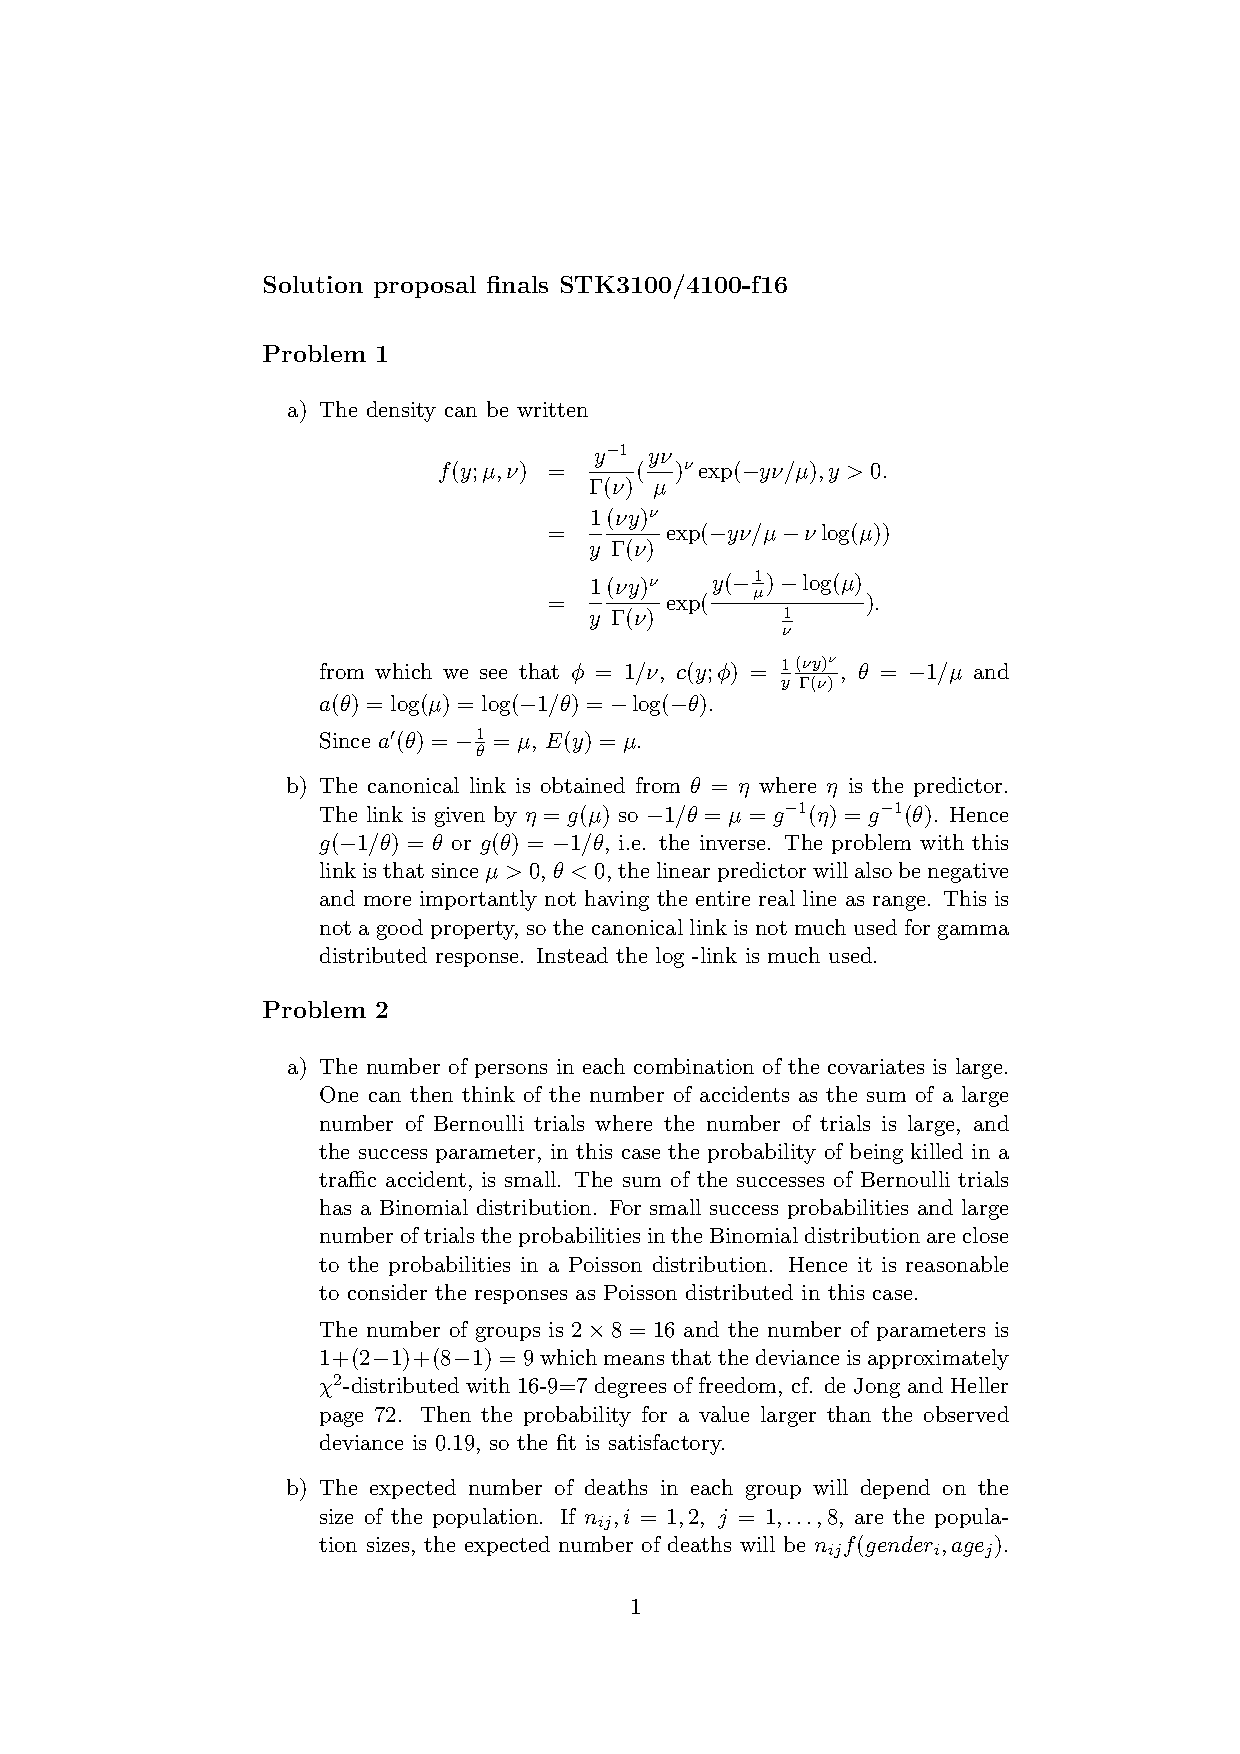
\includepdf[pages = {1}]{exam-exercises/exam-2016-solution.pdf}
\includepdf[pages = {4,5,6,7}]{exam-exercises/exam-2017-solution.pdf}

\printbibliography
\end{document}
